% Sample file on how to use subfiles.
\documentclass[ExampleMasters.tex]{subfiles}

\begin{document}
\clearpage
{\pagestyle{empty}\cleardoublepage}%


\chapter{Hardware architecture(9 Seiten)}
\label{chap:hardware_setup}

\section{Hardware overview}

As already outlined in chapter \ref{chap:overview} the \gls{HCT} vehicles consists of a truck with two semi-trailers. To achieve the goals of this thesis, some modifications had to be done to the combination as well as equipment mounted in addition to the legacy fixtures. The utilized combination can be seen in figure \ref{fig:combination_overview_with_positions}, the shown number will be referenced further-on to give easier insight into the implemented systems' mounting points.

\begin{figure*}[!htb]
	\centering
	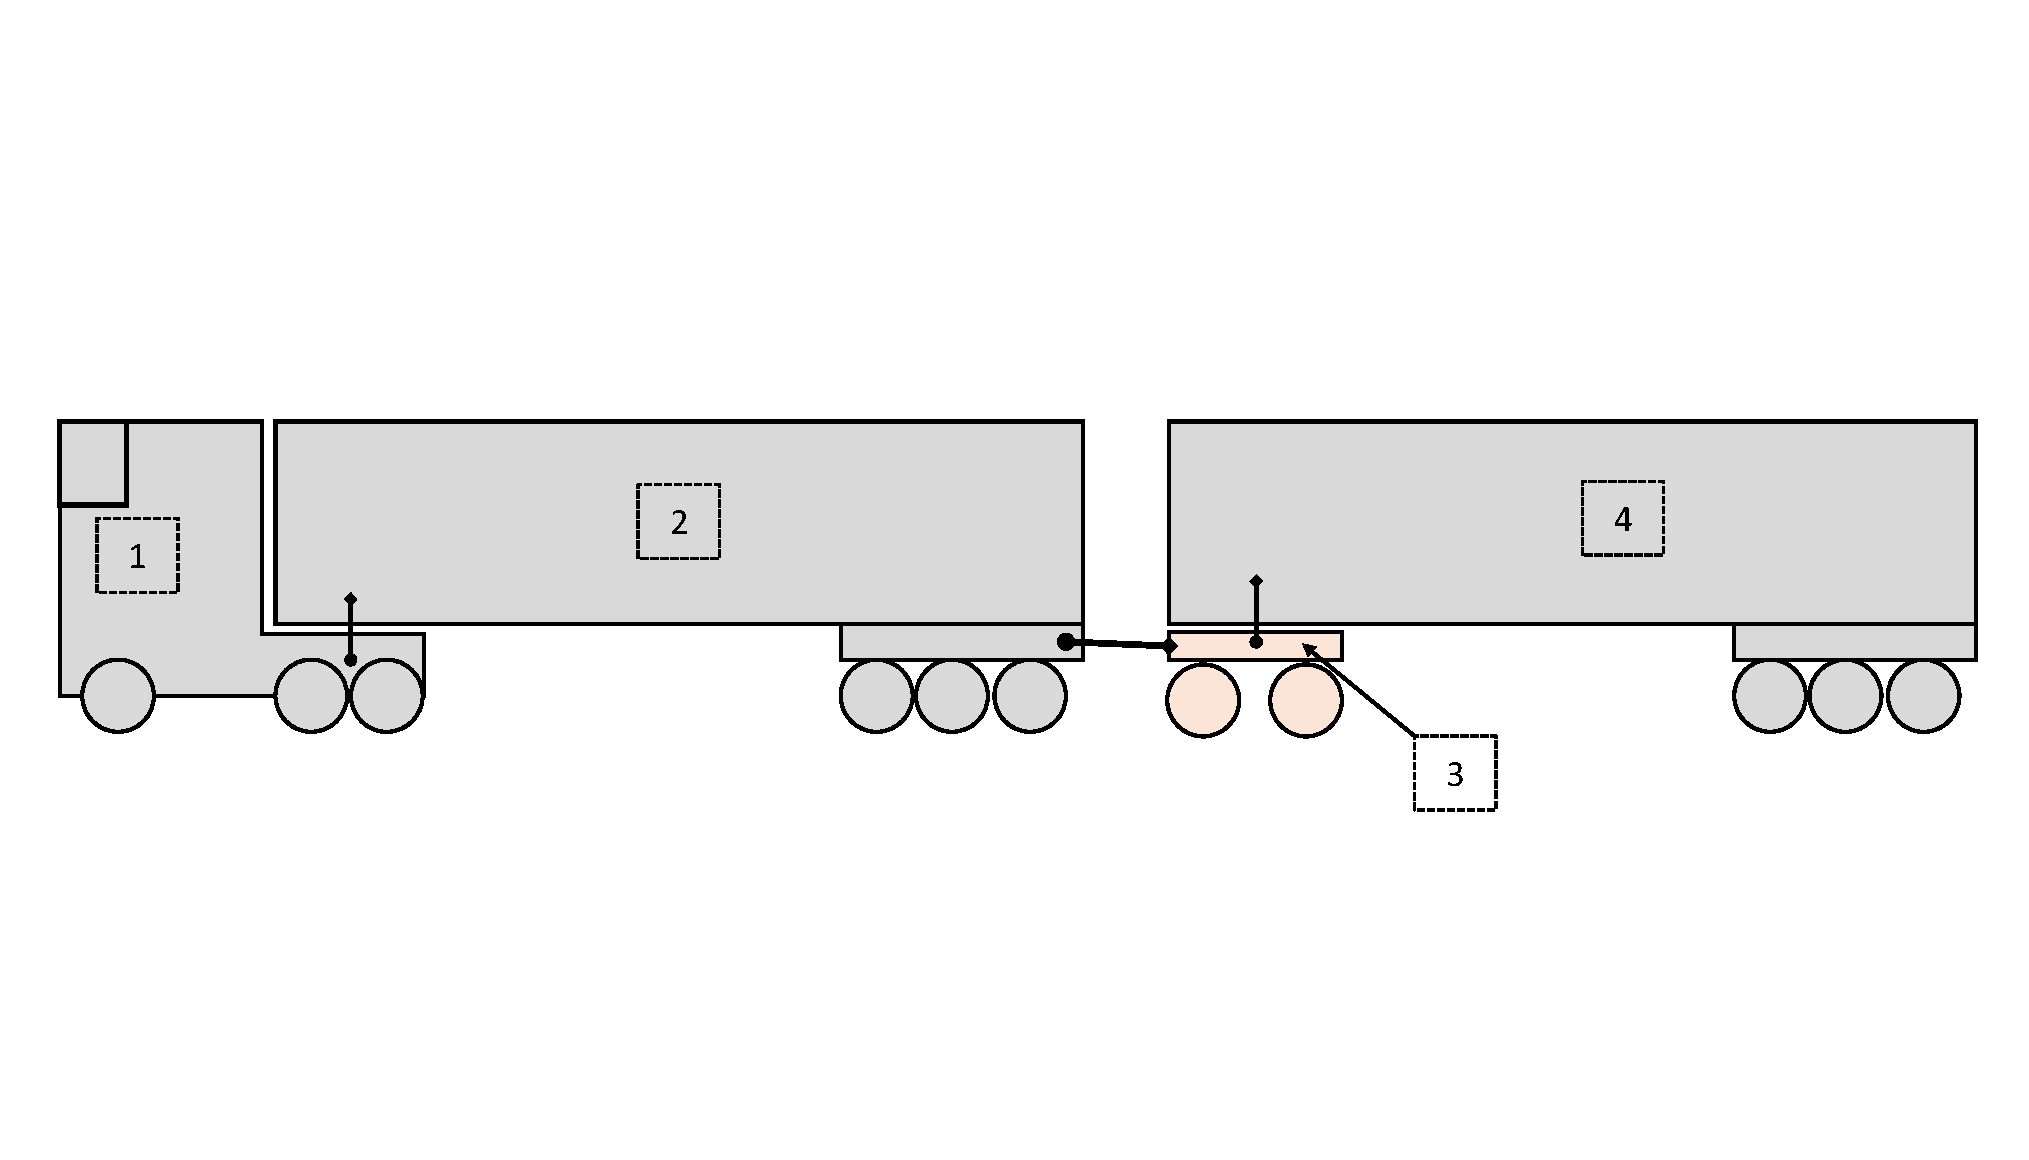
\includegraphics[width=1\linewidth]{figures/combination_overview_with_positions}
	\caption{Positioning of different sensors on the \gls{HCT} vehicle}
	\label{fig:combination_overview_with_positions}
\end{figure*}


The first semi-trailer's (number 2 in figure \ref{fig:combination_overview_with_positions}) rear needs to be equipped with a drawbar eye to accommodate the dolly's drawbar. Besides this obvious physical requirement power supply for the dolly and second trailer, pressurized air hoses for brake actuation, e-brake CAN-buses and lighting connectors have to be routed through the first trailer and supplied to the second trailer with a robust enough cable. This solution had to mainly be custom-made, as these appliances usually would not be available in the rear of a semi-trailer as usually no further towed unit is present. These installations would also apply for any passive combination or for the legacy \gls{VSE} \gls{ETS} system. Furthermore \gls{CAN}s have to be patched through the first semi-trailer (see section \ref{sec:interface_with_truck}). The Real-Time system will be mounted on the dolly directly (position 3) to ensure short signal pathes and minimize wiring efforts. However the Host-PC will have to sit in the tractor (position 1) to sufficiently protect it against the track environment, which would be impossible if sitting on the dolly directly. This leads to an additional ethernet-cable for the Host-PC connection in the cabin which also needs to be routed through the first semi-trailer. The second semi-trailer does not require these modifications, as it is merely a passively towed unit.

Figure \ref{fig:combination_overview_with_positions} also depicts another important aspect. Round bullets on the unit-connecting lines indicate a connection with one rotational degree of freedom (DOF) square bullets mean fixed connection. As \gls{CAN} be gathered from the figure there are three DOF in the whole combination: between tractor and firstsemi-trailer, between first-semitrailer and the dolly, and between the dolly and the second semi-trailer. As the angle between the different units greatly influences the steering performance of combination, the angles have to be accounted for in the simulation and of course also the steering algorithm. It is thus necessary to measure them and provide the measurings via \gls{CAN} to the rapid-prototyping system which is described in great detail in section \ref{sec:interface_with_real_time} for the model-side and in section \ref{fig:dolly_interfaces} for the hardware details. These articulation angle sensors also need to be wired from their mounting point to the dolly, where they are fed into the RapidPrototyping environment. 


\section{Utilized dolly system}
\label{sec:dolly_system}
The utilized dolly by Parator Industri AB (Parator) is equipped with two steerable axles. They are controlled by an after-market solution called \gls{ETS} supplied by \gls{VSE}, of which figure \ref{fig:legacy_system_vse} gives an overview.
\begin{figure*}[!htb]
	\centering
	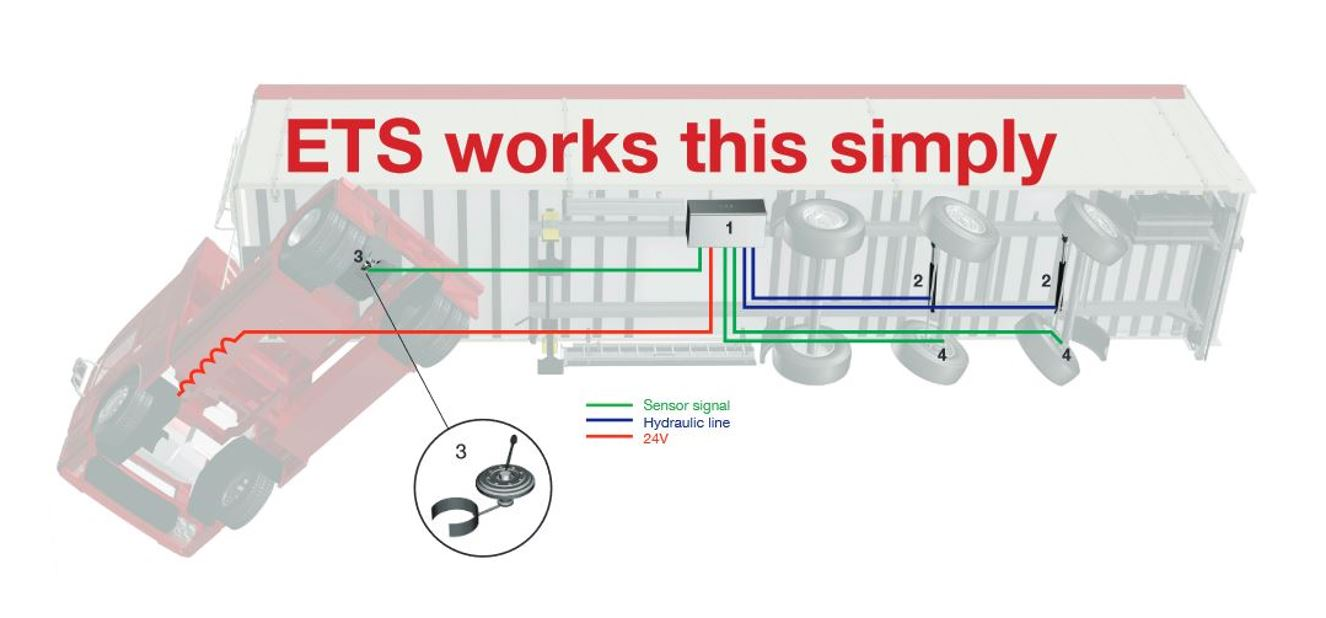
\includegraphics[width=1.0\linewidth]{figures/legacy_system_vse}
	\caption{Active dolly legacy steering system supplied by VSE\cite{dolly_datasheet}}
	\label{fig:legacy_system_vse}
\end{figure*} \\
 Their product includes sensors, \gls{ECU}s and hydraulic systems which come in a ready-to-mount housing, which is placed on the trailer/dolly. This solution is usually sold as a low-speed active steering system for truck-trailer combinations to provide better maneuverability at low speeds in inner-city areas. Besides electrical power and compressed-air (see "2" in the figure) supply there is no connection with the truck in place. This allows for use with many different truck/trailer \gls{OEM}, as no insight into proprietary \gls{CAN} is needed. In the original \gls{VSE} system the two parameters that influence the actuation of the dolly's steering are vehicle speed ("4") and kingpin-deflection ("3"). This deflection is the angle between the truck and trailer, which is measured by an additional kingpin-angle sensor supplied by \gls{VSE} and mounted in the eye of the kingpin hub. Furthermore every steering-knuckle of the dolly is equipped with an angle sensor to provide appropriate wheel-individual feedback for the \gls{VSE} control-system. A diagnosis screen is available in the \gls{VSE}-unit, which allows for relatively simple set-up, calibration and parametrization to be done.\cite{dolly_datasheet} An overview of the implementation of the \gls{ETS}-system in the dolly can be seen in figure \ref{fig:system_overview_ETS}. 
\begin{figure*}[!htb]
	\centering
	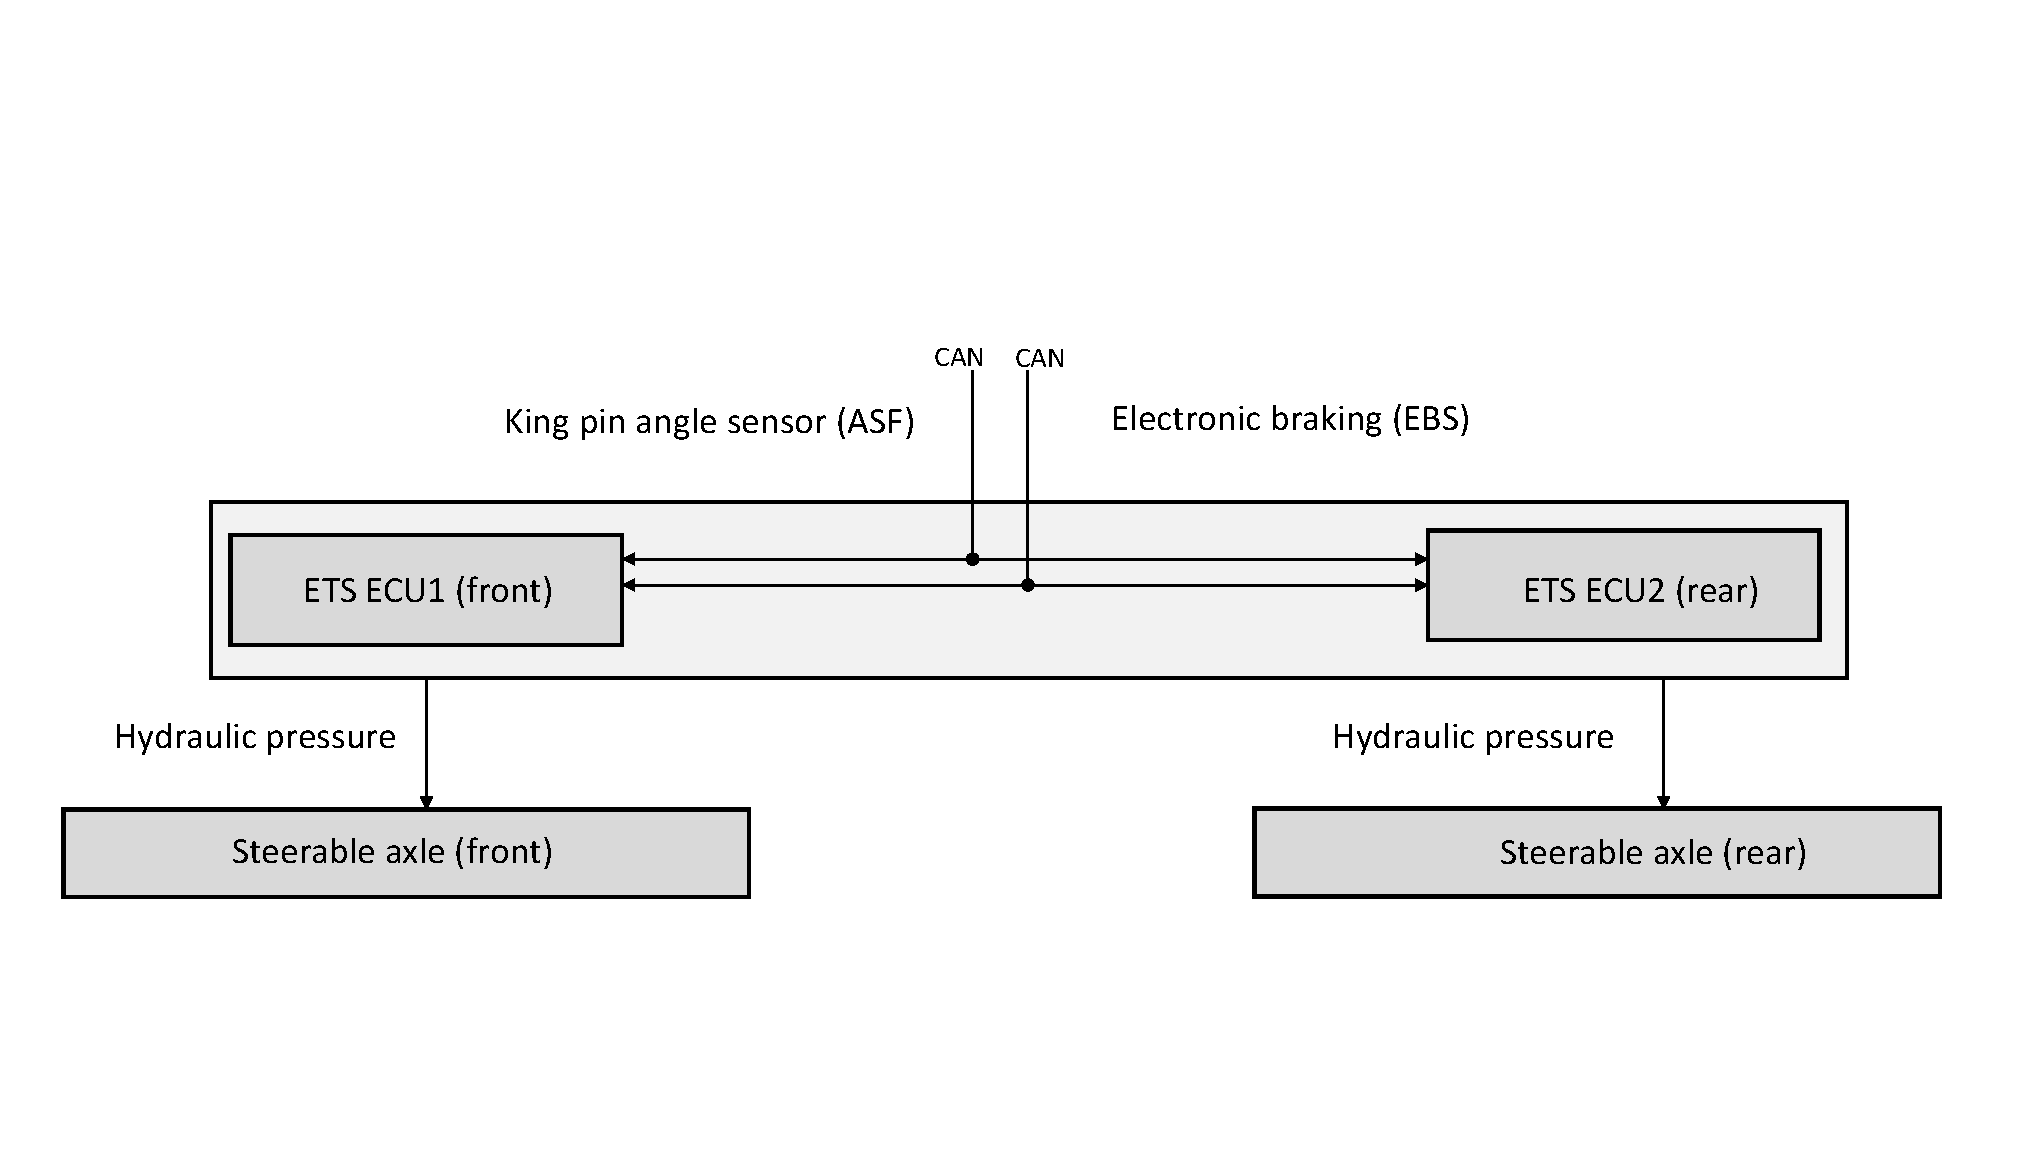
\includegraphics[width=1\linewidth]{figures/system_overview_ETS}
	
	\caption{System overview for sensors and signal path for \gls{ETS} legacy system by VSE}
	\label{fig:system_overview_ETS}
\end{figure*}


VSE provides assisted steering up to a speed of 25km/h over which the possible steering angle is limited until it reaches zero at 55km/h. At this threshold the steerable axles are locked and thus behave like normal rigid axles. This according to the manufacturer is to ensure stability at higher speeds.\cite{dolly_datasheet} Locking the steering at higher speeds leads to a more predictable behaviour for the user and system robustness. However, performance during high speed maneuvers be improved by uniformly steering the dolly as well.\cite{performance_improvement} The desired demonstration of the algorithm presented in chapter \ref{chap:steering_model} will as outlined in the introduction to this thesis, include steering at higher speeds, thus a work-around had to be established.\\
Table \ref{tab:dolly_prop} provides an overview of the properties of the dolly.

\begin{table}[!htb]
	\centering
	\caption{Properties of dolly}
	\label{tab:dolly_prop}
	\begin{tabular}{l r}
		Length   & 6192 mm   \\ 
		Width   &       2600 mm     \\
		Maximum load total   &      18,000 kg   \\
		Maximum load front axle &      9,000 kg      \\
		Maximum load rear axle& 9,000 kg  \\
		Maximum load drawbar& 500 kg  \\
		Maximum load fifth wheel& 18,000 kg  \\
	\end{tabular} \\
\end{table}


\section{Interfaces and connections with dolly}
\label{sec:interface_with_dolly}
Figure \ref{fig:dolly_interfaces} gives an overview of all the in- and outputs of the dolly.\\

\begin{figure*}[!htb]

	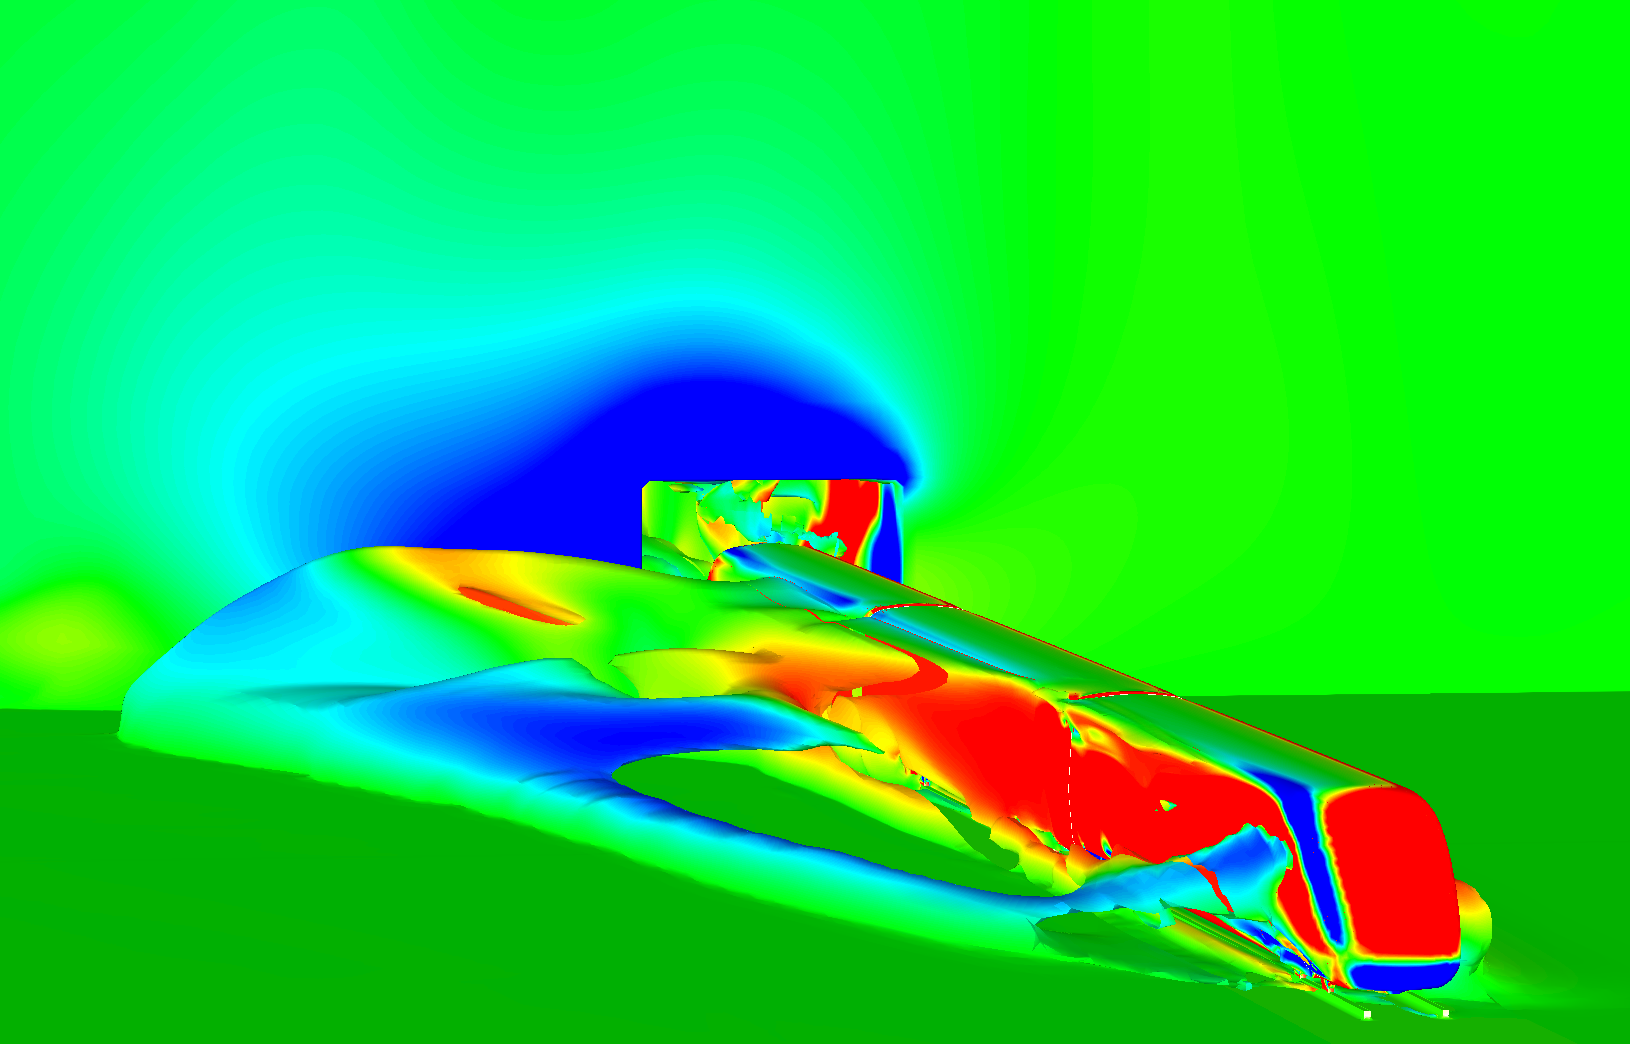
\includegraphics[width=1.3\linewidth]{figures/ExampleCover}
	\caption{Dolly Interfaces}
	\label{fig:dolly_interfaces}
\end{figure*}

To the first semitrailer the dolly is connected with a standard 7-pin ISO 7638-2 connector. This connector includes 24 V electrical power, a signal for \gls{ABS} fault detection as well as the ISO 11992 CAN.
There's a second connector, which includes different pins for different kinds of lighting of the dolly, like the turn indicators and brake light.
The dolly also receives compressed air from the first semitrailer.
For controlling the \gls{MABII} an Ethernet connection is established between the dolly and the tractor unit, where a laptop is located. 
The interfaces of the dolly with the second semitrailer are the same as those to the first one.  
To control and measure signals of the dolly a connection to the dolly's \gls{ETS}- and \gls{EBS} had to be established. To achieve this, different kinds of \gls{CAN}-buses had to be used. That was necessary because the various systems of the dolly use different CAN-protocols. In total five \gls{CAN}-buses connect the \gls{MABII} with the dolly. Two for each of the \gls{ETS}-\gls{ECU}s and one for the \gls{ASF}- and \gls{EBS}-Signal.


One of the \gls{CAN}-buses contains the signals from the EBS-ECUs and the articulation angle sensor, which measures the angle between the dolly and the first semitrailer. It uses the extended CAN-standard. In the original state this \gls{CAN} is directly routed to the \gls{CAN} of the two \gls{ETS}-\gls{ECU}s (see section \ref{sec:dolly_system}). In order to achieve steering that is both independently from the articulation angle as well as the velocity of the vehicle the connection between the \gls{ASF}/\gls{EBS}-\gls{CAN} and the \gls{CAN} of the \gls{ETS}-\gls{ECU} was cut. Instead the ASF/EBS-\gls{CAN} is connected to the \gls{MABII}. Figure \ref{fig:dolly_split} shows an illustration of that.\\

\begin{figure*}[!htb]
	\centering
	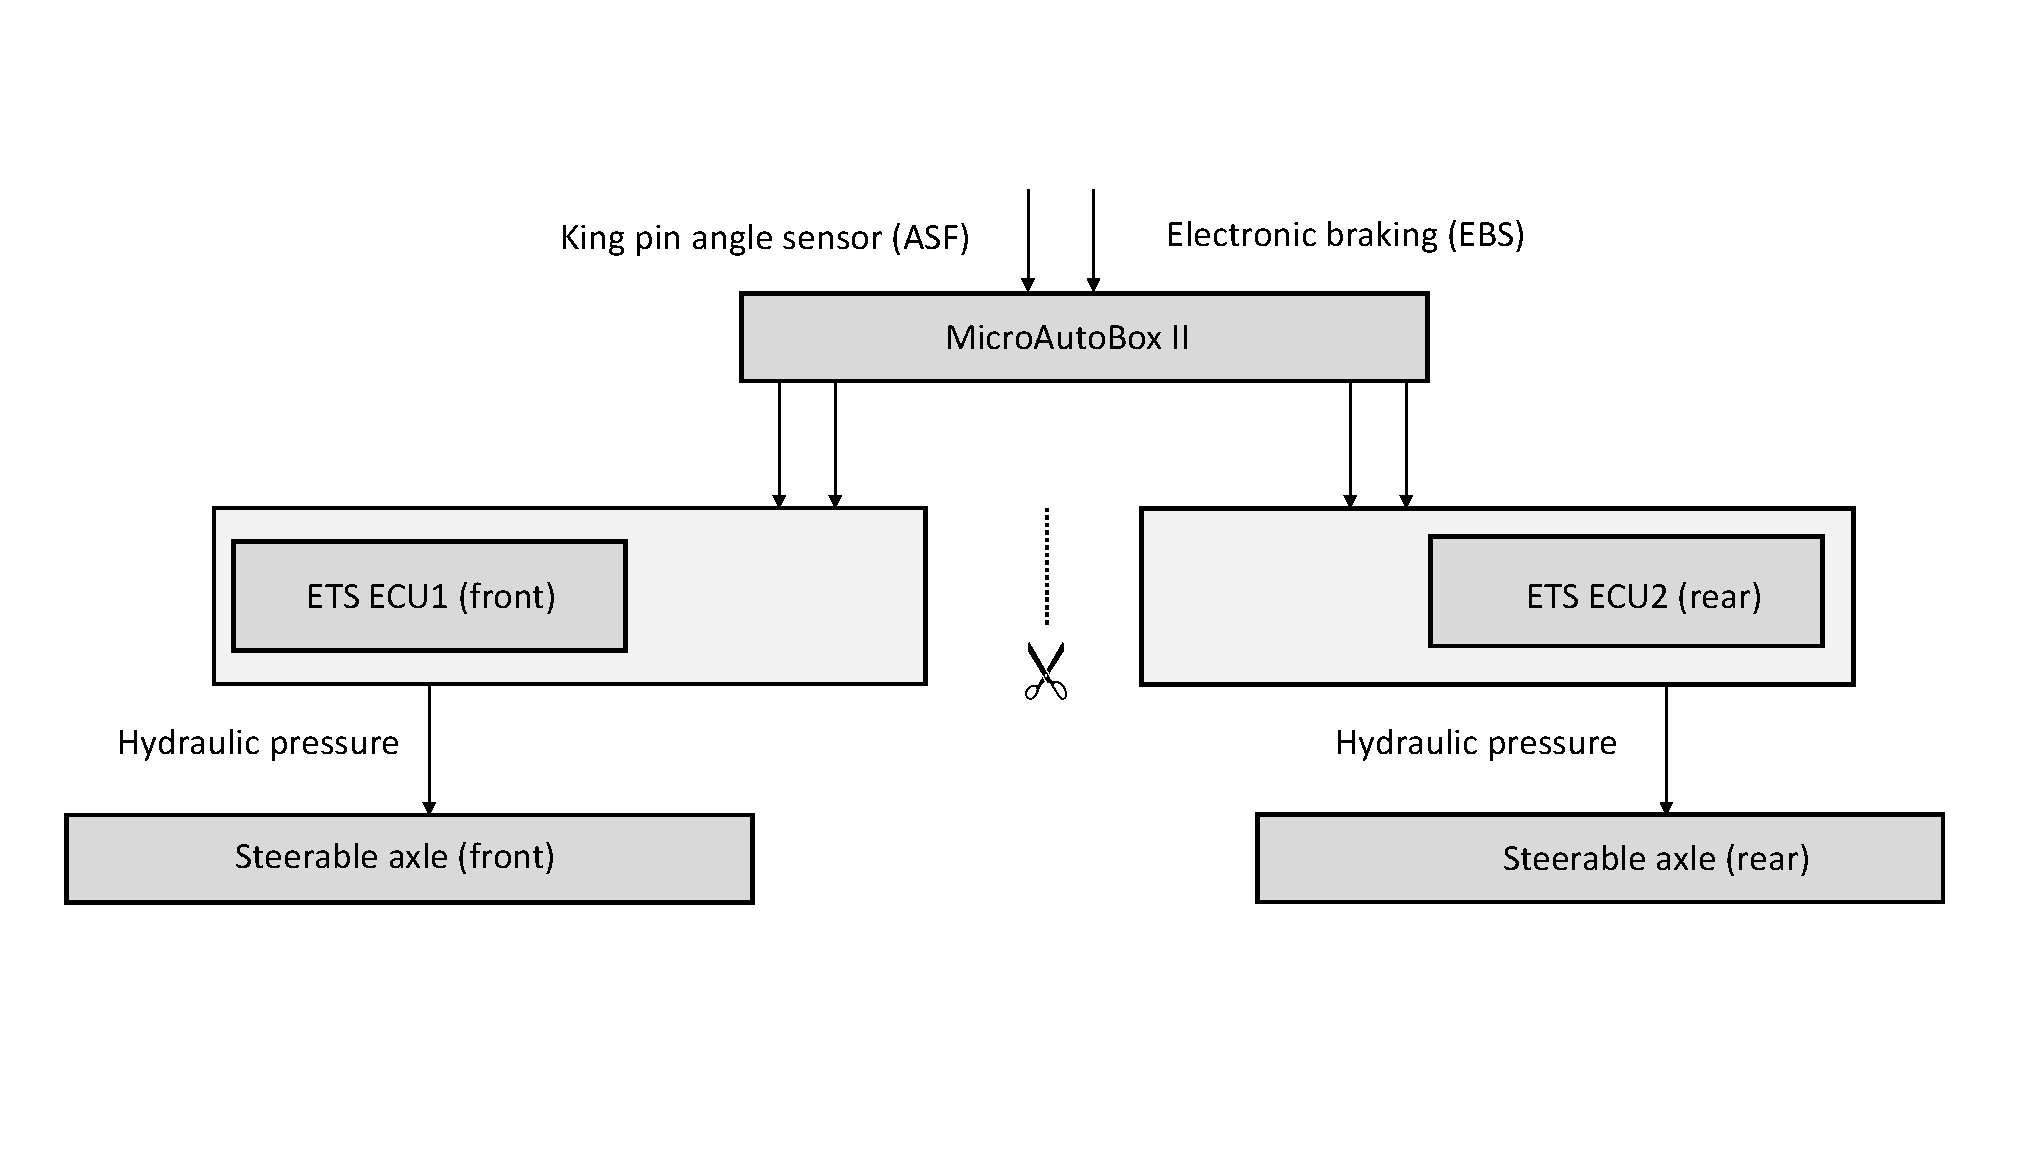
\includegraphics[width=1\linewidth]{figures/dolly_split}
	\caption{Split of \gls{ETS}-\gls{CAN}}
	\label{fig:dolly_split}
\end{figure*}  

The \gls{MABII} is connected to the \gls{CAN} bus of each \gls{ETS}-ECU. Because of the use of different \gls{CAN} standards of the ASF/EBS-\gls{CAN} and the \gls{ETS}-ECU CAN, which uses the J1939 protocol, two physical \gls{CAN} ports are needed on the \gls{MABII} for each \gls{ETS}-\gls{ECU}. Those two \gls{CAN}s are merged inside the breakout-box. Figure \ref{fig:BOB} shows the breakout box which is used to as an interface between the different \gls{CAN}s that were used and the \gls{MABII}. The merging of the two \gls{CAN}s that contain signals for the \gls{ETS}-\gls{ECU} can be seen on the right side of the scheme.\\

\begin{figure*}[!htb]
	\centering
	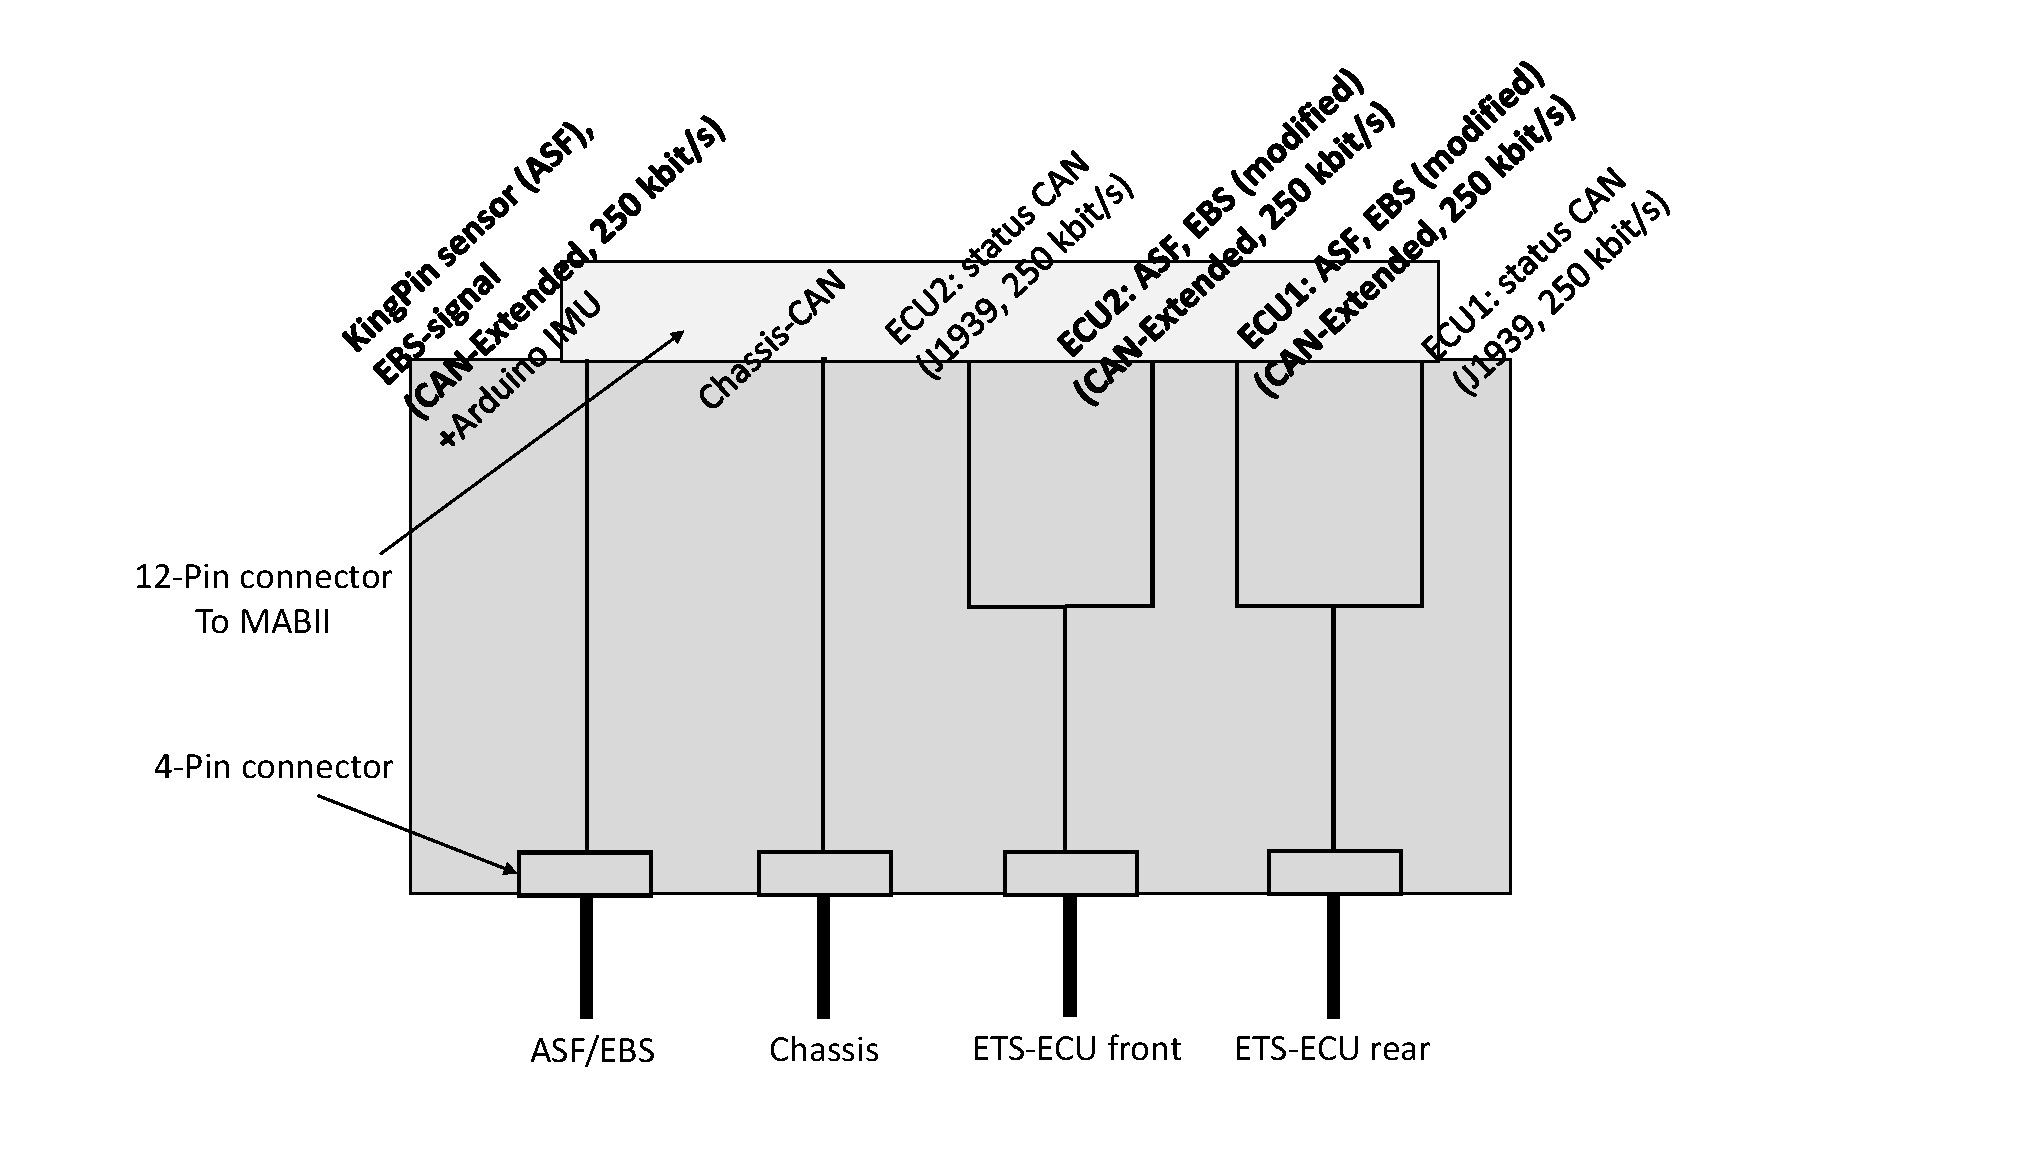
\includegraphics[width=1\linewidth]{figures/BOB_schema}
	\caption{Breakout box scheme}
	\label{fig:BOB}
\end{figure*}


	Furthermore there is the ISO 11992 \gls{CAN} bus which is used for communication between tractor and the attached semitrailers. In the current design this \gls{CAN} is only connected to the EBS-units of the dolly. For future projects it is preferable to connect the \gls{MABII} to that \gls{CAN}, too. If the connection is established and a matching dbc-file for the ISO 11992 standard is acquired, there would be different benefits. For one thing more information about the state of the trailers, like for example axle loads and wheel speeds, could be received and used to improve quality of the capability-state of the dolly (see section \ref{sec:maxi_capabilities}), for another thing there would be the possibility to also control breaking and the leveling of the air suspension of the dolly. With this a more sophisticated control of the vehicle dynamics of the dolly \gls{CAN} be achieved.\\	

\section{Interfaces with truck}
\label{sec:interface_with_truck}
The vehicle model controllers depend on inputs from the tractor unit(see section \ref{chap:steering_model}). One of the inputs is the steering angle of the tractors front axle, another the current vehicle speed. For track-testing the \gls{MABII} is connected to the Chassis \gls{CAN} of the tractor, in order to get those signals. Since the chassis \gls{CAN} of the tractor is not usually available on trailers, the chassis \gls{CAN} needs to be accessed somewhere in the tractor and looped through all the way to the dolly.   
For the \gls{HIL} -testing the tractor unit is simulated using \gls{VTM}  (see section \ref{sec:VTM}). As already mentioned in section \ref{sec:interface_with_dolly} the dolly gets power supply and compressed air indirectly from the tractor over the first semitrailer.

\section{Arduino Due}
\label{sec:arduino}

The Arduino platform series was developed by  SmartProjects company in Italy and consists of a micro-controller board with several in- and output pins, and a set of programming tools to program said micro-controller (see also section \ref{sec:arduino_applications}). Hardware layouts as well as software of this solution are released under an open-source licence, so changes at any level of detail can be made and many other suppliers are now offering solution that tie in with the Arduino. Furthermore this lead to a broad user base and availability of vast supporting resources. For a number of tasks in this thesis, it was decided to rely on this cost-efficient and flexible microcontroller platform. Namely those purposes are:

\begin{itemize}	
	\item data collection from \gls{IMU} and transmission over CAN
	\item CAN-to-UDP gateway
	\item CAN-to-Serial gateway for \gls{HIL} -testing
	\item benchtesting sensor outputs and quick CAN-debugging
\end{itemize}

SmartProjects offers various Arduino boards mainly differing in number of communication pins, memory size, clock frequency and physical size. It was decided to utilize the to date most powerful Arduino Due, offering 84 MHz of clock-speed on a ARM Cortex-M3 processor, 512kB flash memory for program-code and a 96kB working SRAM. It is the first Arduino with 32-bit architecture. This was done in order to allow for future use of this platform in other projects and having enough space for different sub-programs on the controller as well as enough processing power to deal with basic signal filtering and parsing at appropriate speeds. 

The Due has a native \gls{I2C} interface, which was used to gather the measurings from the \gls{IMU}. It also has a \gls{SPI} which is needed to access the ethernet controller necessary for the \gls{CAN}-\Gls{UDP}-gateway (refer to section \ref{sec:can_udp_gateway}), serial communication is also handled on hardware level. The availability of these ports in hardware form allow for robust systems and eliminate the need to implement those protocols on software level (bit-banging), which frees up memory resources. In addition to this digital communication possibilities the Due offers an abundance of 54 digital and 12 analog freely configurable I/O-pins. The Due is also the first Arduino to host an on-board \gls{CAN}-controller, which in this thesis will be used for measurement transfer to the logging system (\gls{MABII}), eliminating the need for additional hardware for \gls{CAN}-bus interfacing on the Arduino side.

Besides the power-supply and the \gls{IMU}-chip a MCP2551 CAN-transceiver by Microchip Technology Inc. was incorporated to take care of the pyhsical layer of CAN-bus communication by converting the digital signals from the Due's CAN-controller to the standardized voltage levels of the \gls{CAN}. The MCP2551 is capable of different \gls{CAN} standards and fully ISO-11898 compatible, which makes future use in different environments or as unit for in-vehicle CAN-interfacing feasible.

The Arduino Due was used to determine the delays in the system (see section \ref{sec:measuring_delay}) as well as a light-weight solution to quickly read \gls{CAN}-outputs of the various systems during this thesis' work. This proofed to be an easy debugging solution. Additionally it was used to trigger some error codes to test the developed safety mechanisms (see section \ref{sec:fault_detect_test}). 

%\begin{itemize}
%\item clock frequency
%\item RAM/ROM
%\item ISP flash
%\item robustness, reliability, cost-effectiveness
%\item input/outputs analog $\&$ digital
%\item native I2C capability
%\item CANcomm except of physical layer/transceiver available (OSI reference!) --$>$ no bit-banging needed --$>$ faster
%\end{itemize}

\section{Real-Time Environment}
\label{sec:realtime_environment}

To run the utilized steering controller outlined in chapter \ref{chap:steering_model}, a \gls{MABII} by dSpace company is utilized, an embedded computer running on a 900MHz PowerPC CPU with 32MB RAM. The \gls{MABII} has very compact dimensions of only 200mm x 225 mm x 50mm making it possible to fit it inside the housing locker of the \gls{VSE} \gls{ETS} (position 3 in figuure \ref{fig:combination_overview_with_positions}). It accepts a wide variety of input currents for power supply, is shock resistant to a high degree and equipped with sturdy \acrshort{LEMO}  connectors; the unit is cast into very robust aluminium housing and has mounting points, so it can be utilized in tougher conditions in automotive applications. It boots up almost at the speed of a standard \gls{ECU} and can run headless ensuring safety, even without the Host-PC to control it. Besides normal digital and analog in- and output pins, CAN, Ethernet and many other standard interfaces are readily available, making for a practical use of these protocols on a high level. 

The connection to the various \gls{CAN}-buses for this thesis' purposes is established via the dSpace \gls{ZIF}-connector. This is a specially made connector that allows to access all of the 64 in- and output-pins of the \gls{MABII} and quickly plug and unplug the \gls{MABII} Ethernet connections with reliable \acrshort{LEMO}  connectors are used to communicate with the Host-PC which runs logging and start-up sequences during testing. Power-supply is realized from the buffer batteries of the hydraulic steering system of the dolly during testing and a standard laptop charger during bench-testing.

The hardware platform is part of an integrated chain of software tools to develop functions and models in the sense of RapidControlPrototyping. It integrates with MATLAB's Simulink and compiles and uploads executable code of the abstract Simulink-models directly into the MABII's program memory. Furthermore a tool (ControlDesk 4.2) to log and manipulate the executed Simulation running on the \gls{MABII} is used on the connected Host-PC. This software tools will be detailed in section \ref{sec:matlab} and \ref{sec:control_desk}.\cite{MABII_product_descr}



\subsection{CAN-bus extension}
\label{sec:can_udp_gateway}
The \gls{MABII} comes with a preset number of in- and output ports. The maximum number of CAN-buses, that can be connected to the \gls{MABII}'s native controllers is limited to six. As there is no off-the-shelf solution by dSpace for extending the available bus-connections, it was necessary to come up with a gateway solution that allows to patch the needed amount of additional \gls{CAN}-buses through to the ethernet connection which is also available on the \gls{MABII}. It should be mentioned that this issue with lacking CAN-buses mainly arises due to the limitation, that buses have to be kept separate as shown in figure \ref{fig:dolly_split}. Without this limitation it would of course be possible to just merge the different physical CAN-bus lines to one line.

A gateway from CAN-protocol to the standardized \gls{UDP} used for communication on Ethernet  infrastructure was implemented to achieve this. It is a very light-weight protocol, that is straight-forward to implement and runs well, even with limited processing power on a microcontroller. For future purposes the broadcasting capabilities of \gls{UDP} might also proof useful, as many nodes could be connected to this \gls{CAN}-to-\gls{UDP} gateway all receiving the broadcasted datagrams for example for visualization on different computers or additional logging outside of the \gls{MABII} environment. One limitation that was decided on, is to have receiving capabilities only for the \gls{MABII} to eliminate the need for extensive computation and CAN-matrix handling on the Arduino. \\


\textit{Excursus: The \gls{CAN}-protocol is the most widespread protocol to allow for communication between different \gls{ECU}s in the automotive field. Development began at the Robert Bosch GmbH, but is now standardized and enhanced and adjusted for special purposes internationally. Messages are broadcasted by the bus-participants and stamped with their unique identifier, which also doubles as an arbitration token to handle message prioritization. Each bus-participant can listen to all available messages and "only picks from the bus what he needs". The standard message has a size of eight bytes \`{a} eight bit, transmitted after the identifier and followed by an ending sequence. Hardware-wise \gls{CAN}-communication relies on only a pair of twisted wires, where a very robust voltage difference signal is transmitted. }\cite{CAN_intro}\\


By utilizing the \gls{UDP}-protocol to acquire data into the simulation, the \gls{MABII} environment's very convenient possibilty to incorporate \gls{CAN} database files (.dbc-file)\footnote{Correlates physical human readable/understable signals with units to the actual distribution over the different bytes of a \gls{CAN}-frame. It allows to "decrypt" the information which is available on a \gls{CAN}-bus and allows to code and send messages in the respective format that the other bus-participants (ECUs, sensors) expect.}, which is the usual way to exchange information and instructions for \gls{CAN}-networks is no longer available. To decompose the \gls{UDP} packets into the original signals it was necessary to implement the function of a .dbc-file in the underlying Simulink-model. 

All messages that the CAN-gateway is supposed to handle and forward are put into one \gls{UDP} frame in succession with respective CAN-identifiers and additional spacer bytes between signals. The \gls{UDP} frame is broadcasted every time a new CAN-message reaches the gateway on one of its \gls{CAN}-buses. Messages that were not updated with the incoming \gls{CAN}-message will be kept at their previous value. This is called for, as \gls{UDP} is a connection-less protocol without any loss-prevention mechanisms like acknowledgment-handling or retransmission of messages. Holding the values if not available ensures, that at least some value is available on the bus. \gls{UDP} also doesn't have native timestamping, which is why a \gls{GPS}-shield was introduced to receive the high-precision time to allow for easy synchronizing of logging over different platforms (\gls{MABII}-environment, \gls{IMU}s, external \gls{CAN}) by adding the global time to each sent packet.

To allow for easier scalability to add more CAN-buses in the future it was decided to not use the Due's two native CAN-controllers but rely on the external MCP2515 in combination with the already mentioned transceiver (MCP2551). As shown in figure \ref{fig:can_extension} it is controlled via \gls{SPI} . More bus-participants \gls{CAN} be added conveniently by incorporating additional instances of these two microships and attaching them to a device selection pin (depicted as SS) each.\\




\begin{figure*}[!htb]
	\centering
	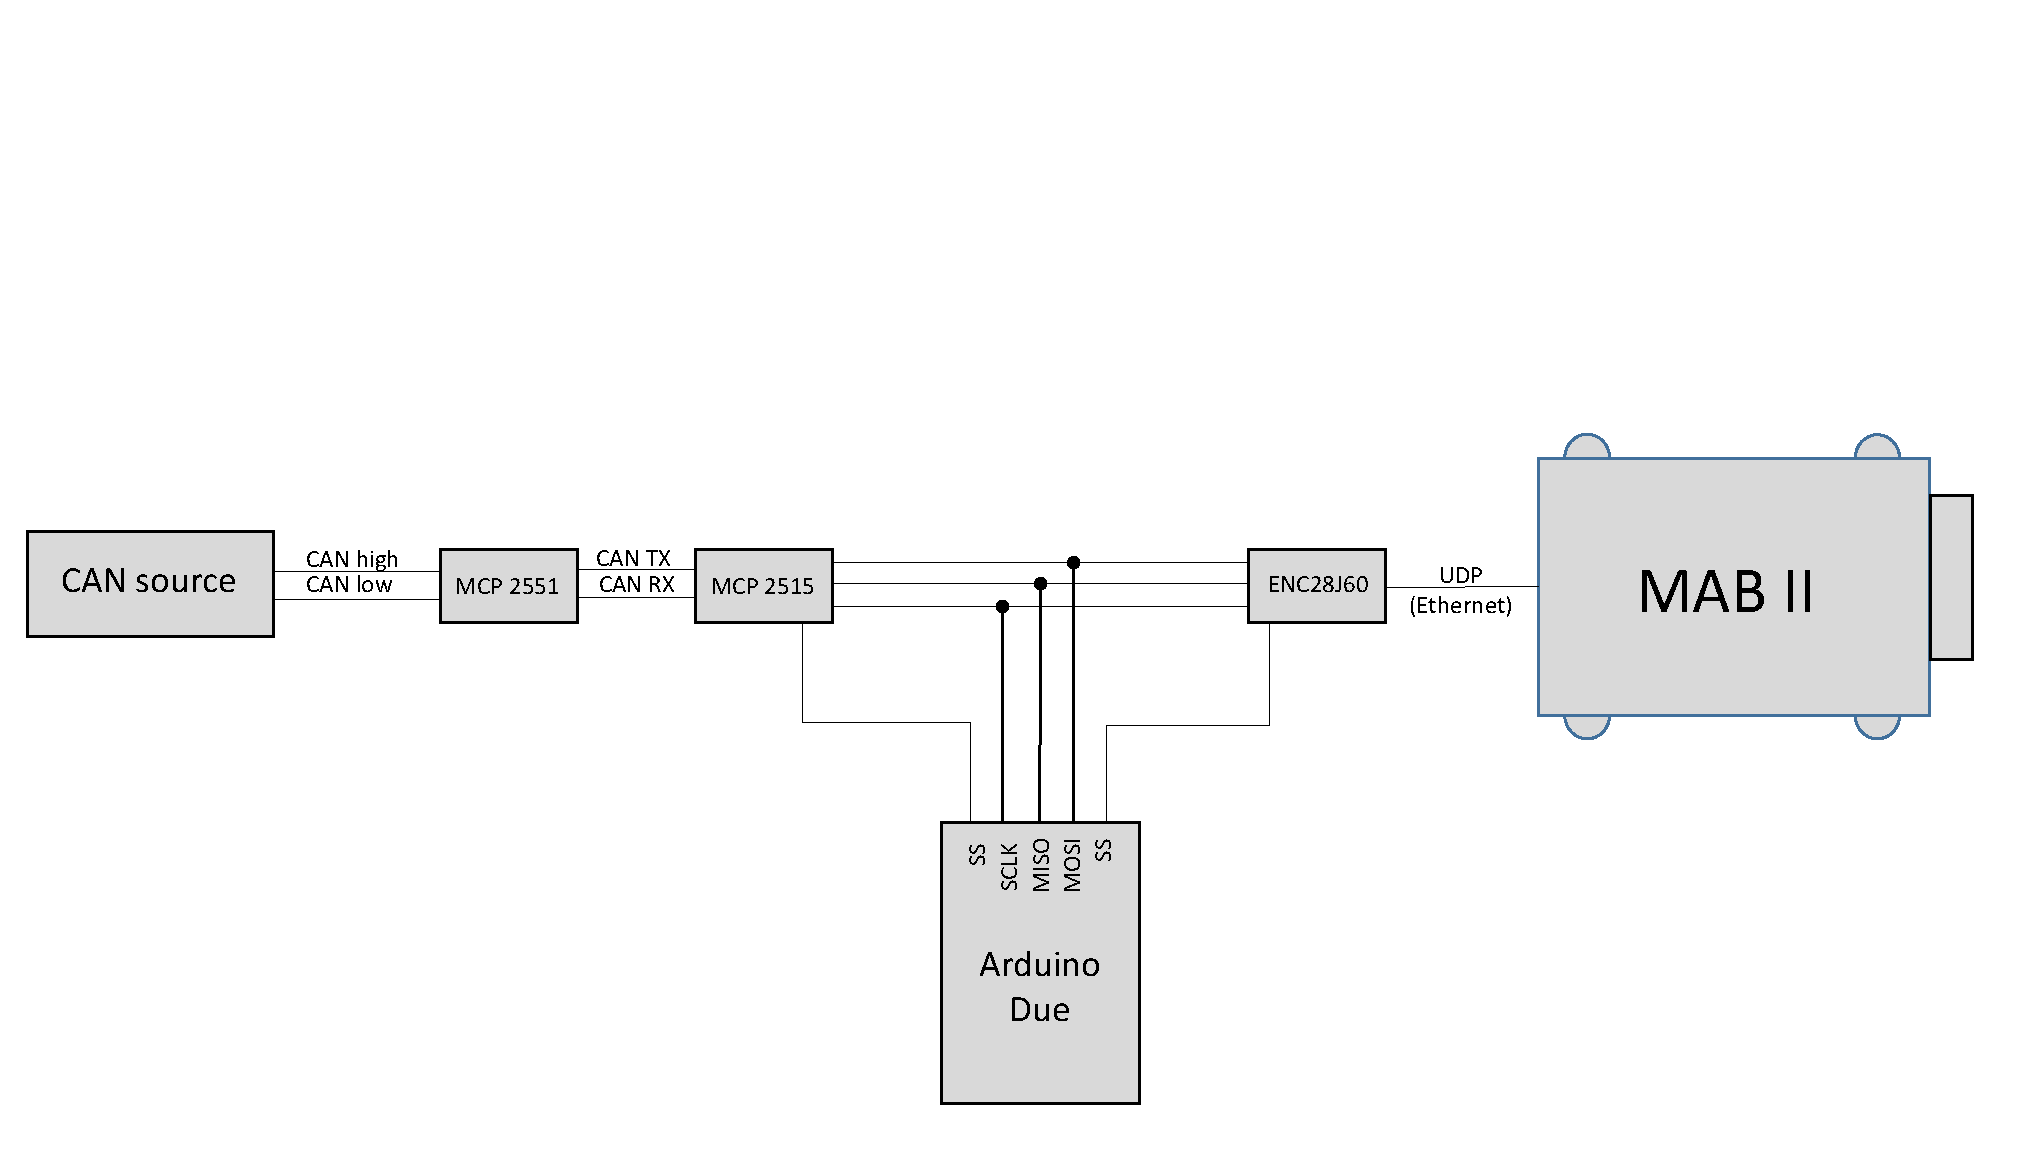
\includegraphics[width=1\linewidth]{figures/can_extension}
	\caption{Extension of \gls{MABII} \gls{CAN}-buses (hardware overview)}
	\label{fig:can_extension}
\end{figure*}


\begin{itemize}
	
	\item daten-konvertierung und packaging zu \gls{UDP} und von \gls{UDP} zu Daten in CD!!
	%\item Skizze des Systems
	\item verwendete bibliotheken
	
\end{itemize}

\section{Measurment Setup}
\label{sec:measurement_setup}

\subsection{On-board sensors}

\begin{table}[!htb]
	\begin{tabular}{llll}
		\textbf{Sensor}       & \textbf{Measurings}                                                 & \textbf{Type} & \textbf{Mounting point} \\
		Draw bar sensor  & \begin{tabular}[c]{@{}l@{}}Articulation angle\\ Temperature\end{tabular} & External      & Draw bar                 \\
		EBS                   & wheel speed                                                         & External      & wheel brakes            \\
		Steering angle sensor & steering angle (first, second axle)                                 & External      & steering knuckles      
	\end{tabular}
	\caption{Available sensors of VSE's ETS}
	\label{tab:ets_sensors}
\end{table}





\subsection{Inertial measurement unit}
\label{sec:IMU}
To determine the processing delays in the control chain (refer to chapter \ref{chap:processing_time_delay}) as well as logging implementation for verification and analyses purposes a number of inertial measurement units (IMU) where utilizied throughout this thesis' work. The system at hand combined a gyroscope (L3GD20H), and an accelero- and magnetometer (LSM303D) into an \gls{IMU} put on one circuit board.\cite{IMU_homepage_shop} This one-chip solution allowed for a convenient access to the sensor measurings, as the sensor outputs could be received via Inter-Integrated Circuit-protocol (I$^{2}$C)  which eliminates the need for a transducer. Furthermore a high-pass filter is integrated into the \gls{IMU}'s accelerometer, which leads to simpler compensation of the immanent drift of the magnetormeter. These units supply the measurings for three axes each at a maximum frequency of 1600Hz for the accelerometer and 757.6Hz for the gyroscope.  \cite{accelerometer_datasheet}\cite{gyrometer_datasheet}

The \gls{IMU}-chip was put in a suitable plastic housing and cast into resin, to fixate the \gls{IMU} securily and prevent movement relative to the truck-frame on which it will is mounted as well as ensuring water-proofing.

Figure \ref{fig:IMU_overview} shows, how the \gls{IMU} is connected to the Arduino Due utilizing the \gls{I2C}-interface on the Due. Not pictured are the power supplies (both 5V) for the MCP2515 \gls{CAN}-transceiver and the \gls{IMU} itself. To minimize cables that have to be rooted through the combination and avoid problems with cable length for the power cables, it was decided to equip each of these assemblies with a rechargeable battery-pack. This also allows to measure in remote location and collect data locally on the Arduino Due during testing, eliminating the need for CAN-communication completely if needed in the future.

A maximum of two \gls{IMU}s \gls{CAN} run on one \gls{I2C} line as it is possible to override the last bit of the otherwise hard-coded \gls{I2C} address via a hardware jumper. If both \gls{I2C} lines of the Due are used, it would be possible to connect up to four IMUs to one Arduino. Though eight \gls{IMU}s are desired for the whole \gls{HCT} vehicle, this was outruled as a possibility for this project, due to the limitations of the physical bus-length of the \gls{I2C} lines of only a few meters (as the name already suggests \gls{I2C} is not meant for long distance communication). As \gls{CAN} also be seen in the overview figure of the setup on the truck in figure \ref{fig:combination_overview_with_positions} this distance would be exceeded with the distance between the different mounting points (15-20m).

In the final measuring setup the assembly shown in figure \ref{fig:IMU_overview} will be present four times in the whole combination, to gather motion data from each independently moving part. Figure \ref{fig:combination_overview_with_positions} shows those placements in an overview sketch. The correct placement will be as close as possible to the \gls{COG} of the respective unit to have as little influence of the vehicle's rotary motions as possible, which drastically reduces work in  data analysis further on. \gls{COG}  locations \gls{CAN} be gathered from Volvo's internal database and are available at the test site. Putting two \gls{IMU}s in each spot allows for averaging and ensure redundancy should one \gls{IMU} chip fail or produce corrupt outputs, which occured from time to time during the bench-testing of the assembly if the voltage of the preliminary power-supply dropped due to other loads.\\

\begin{figure*}[!htb]
\centering
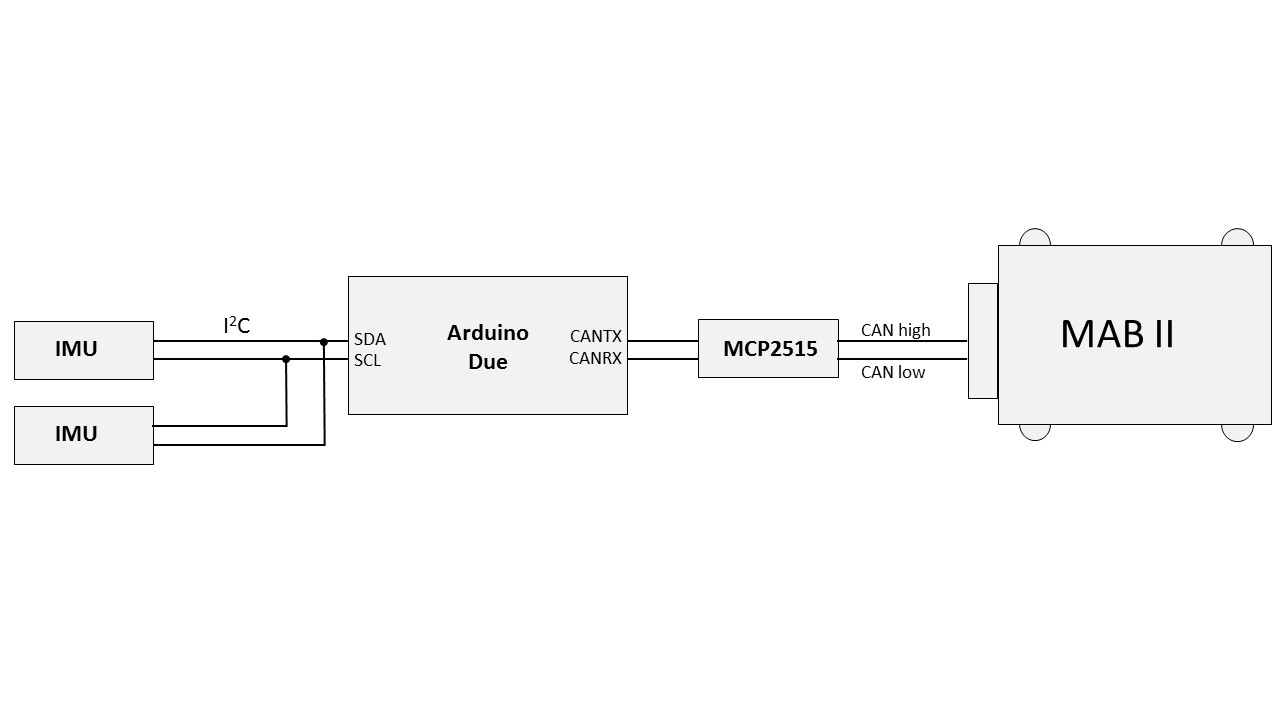
\includegraphics[width=1\linewidth]{figures/IMU_overview}
\caption{Connection of \gls{IMU} with Arudino Due to \gls{MABII}}
\label{fig:IMU_overview}
\end{figure*}






\end{document}
